\chapter[Detailed Design of Agentic Logistic Mitigation Framework]{Detailed Design of Agentic Logistic Mitigation Framework}

The detailed design of the proposed system is presented here. The internal organisation of modules, the workflow of system operations, the database structure, interface design, and the detailed interaction between components are explained herein. Unlike the High-Level Design chapter, which focuses on the overall architecture and conceptual organisation of the system, this section focuses on the internal structural and functional design of the system components.


\section[Structure Chart]{Structure Chart}
This section presents the structural decomposition and organization of the system into modules and sub-modules. By breaking the digital twin application down into self-contained components, we ensure high cohesion and low coupling across the codebase. The functional divisions and control hierarchy are detailed in the following subsections.
\subsection[Functional Decomposition]{Functional Decomposition}
To manage complexity, the system is decomposed into four distinct, logical modules. Each module encapsulates a specific domain of operations, ensuring high cohesion and low coupling.

\subsubsection{A. Friction Sentry Module}
\textbf{i. Purpose} \\
This module is responsible for the ingestion, parsing, and structured interpretation of disruption signals. It serves as the risk-monitoring interface that maps raw event alerts to concrete physical impacts.

\textbf{ii. Contribution to Overall System} \\
It protects the downstream optimization algorithms from dealing with raw text or unstructured data by translating news signals into standardized variables (severity multipliers, location targets, and cost impacts).
\subsection[Module Hierarchy]{Module Hierarchy}
The system is organized into a modular control hierarchy where responsibilities are distributed between the user interface, the API orchestration layer, and local computation engines, as illustrated in Figure~\ref{fig:hierarchy}.

\begin{figure}[htbp]
    \centering
    \makebox[\textwidth][c]{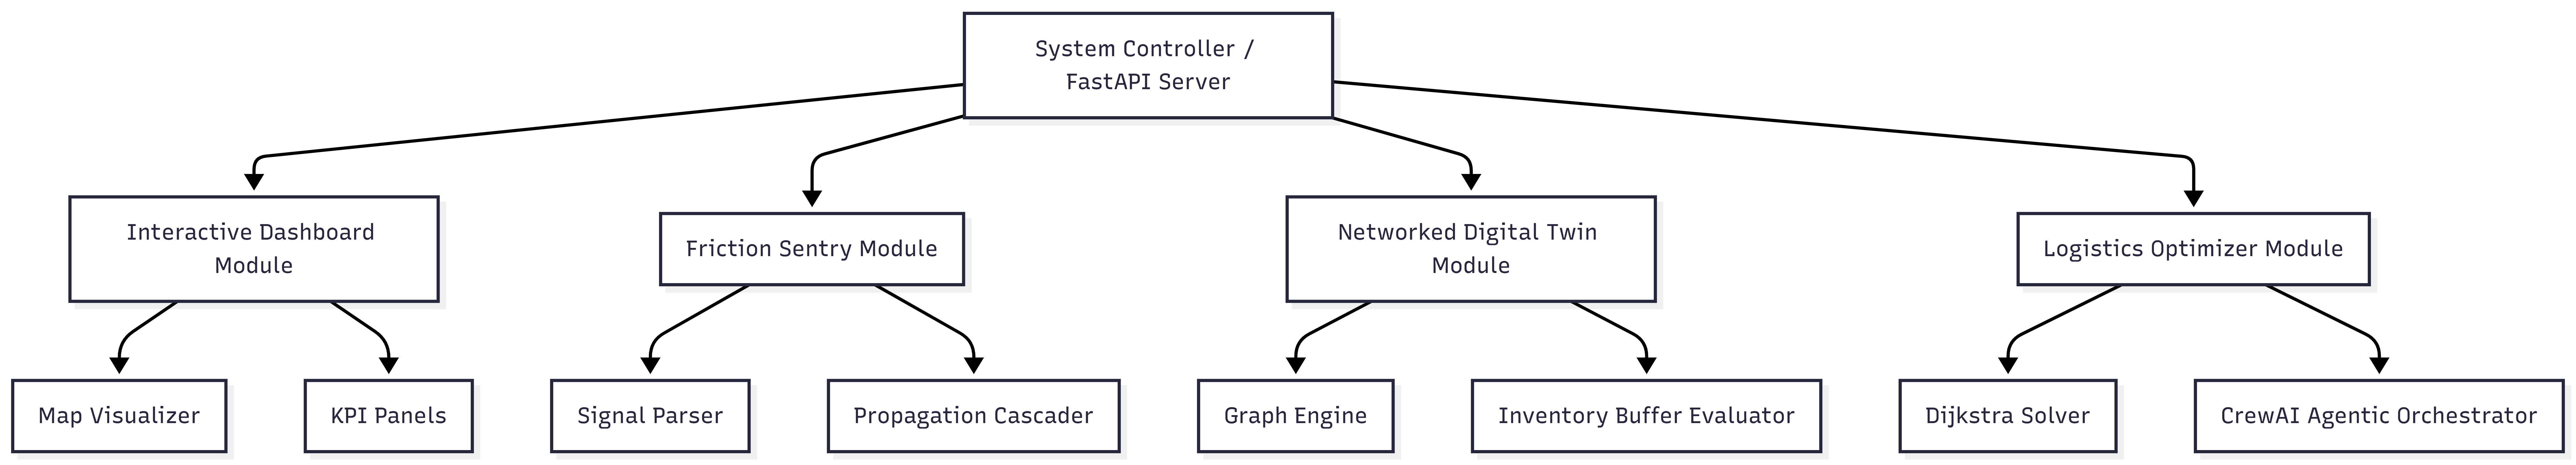
\includegraphics[width=1.1\textwidth]{Figures/Module hierarchy.png}}
    \caption{System Module Hierarchy and Control Structure}
    \label{fig:hierarchy}
\end{figure}

\begin{itemize}
    \item \textbf{Parent-Child Relationships:} The FastAPI Server acts as the central controller orchestration parent. It accepts inputs from the frontend Interactive Dashboard, coordinates signal transformations inside the Friction Sentry, updates network parameters inside the Networked Digital Twin, and executes path-finding inside the Logistics Optimizer.
    \item \textbf{Control Hierarchy:} Operations are strictly top-down. The user initiates requests from the Interactive Dashboard (Child). The FastAPI Controller (Parent) intercepts the request, routes it sequentially through the computing modules, and returns the unified response.
    \item \textbf{Distribution of Responsibilities:}
    \begin{itemize}
        \item \textbf{Frontend:} Handles user interaction, rendering Leaflet coordinates, and strategy state.
        \item \textbf{Backend API Layer:} Manages execution flow, processes HTTP inputs, and parses JSON parameters.
        \item \textbf{Algorithmic/Agentic Engine:} Resolves mathematical routing and handles multi-agent reasoning loops.
    \end{itemize}
\end{itemize}
\subsubsection{A. Networked Digital Twin Module}
\textbf{i. Purpose} \\
This module maintains the in-memory representation of the logistics network (directed graph topology) and models inventory health. It simulates the physical reaction of the supply chain network when a shock is injected.

\textbf{ii. Contribution to Overall System} \\
It computes the real-world impact of delays on safety stock and inventory levels. By calculating stockout risks and daily consumption depletion, it provides the operational context needed to trigger emergency actions.

\subsubsection{B. Logistics Optimizer Module}
\textbf{i. Purpose} \\
This module serves as the execution and decision-making engine of the system, responsible for mathematical path routing and orchestrating autonomous LLM agents to resolve supply chain exceptions.

\textbf{ii. Contribution to Overall System} \\
It acts as the system's brain. It calculates alternate paths bypassing disruptions, coordinates agent tasks (Optimizer, Analyst, and Communicator), and executes corrective replenishment actions to prevent stockouts.

\subsubsection{C. Interactive Dashboard Module}
\textbf{i. Purpose} \\
This module provides the user interface (UI) to visualize the state of the logistics network, display alternate route simulations, and present comparative benchmark metrics.

\textbf{ii. Contribution to Overall System} \\
It makes the complex underlying data understandable to human operators by overlaying geographic routes on a map, displaying stockout warnings, and highlighting the cost and time savings of agentic optimization versus the human baseline.


\section[Module Interaction Flow]{Module Interaction Flow}
Modules interact asynchronously and sequentially to process disruptions and update the digital twin. Figure~\ref{fig:interaction_flow} depicts the sequential flow of data and control signals across the system components.

\begin{figure}[htbp]
    \centering
    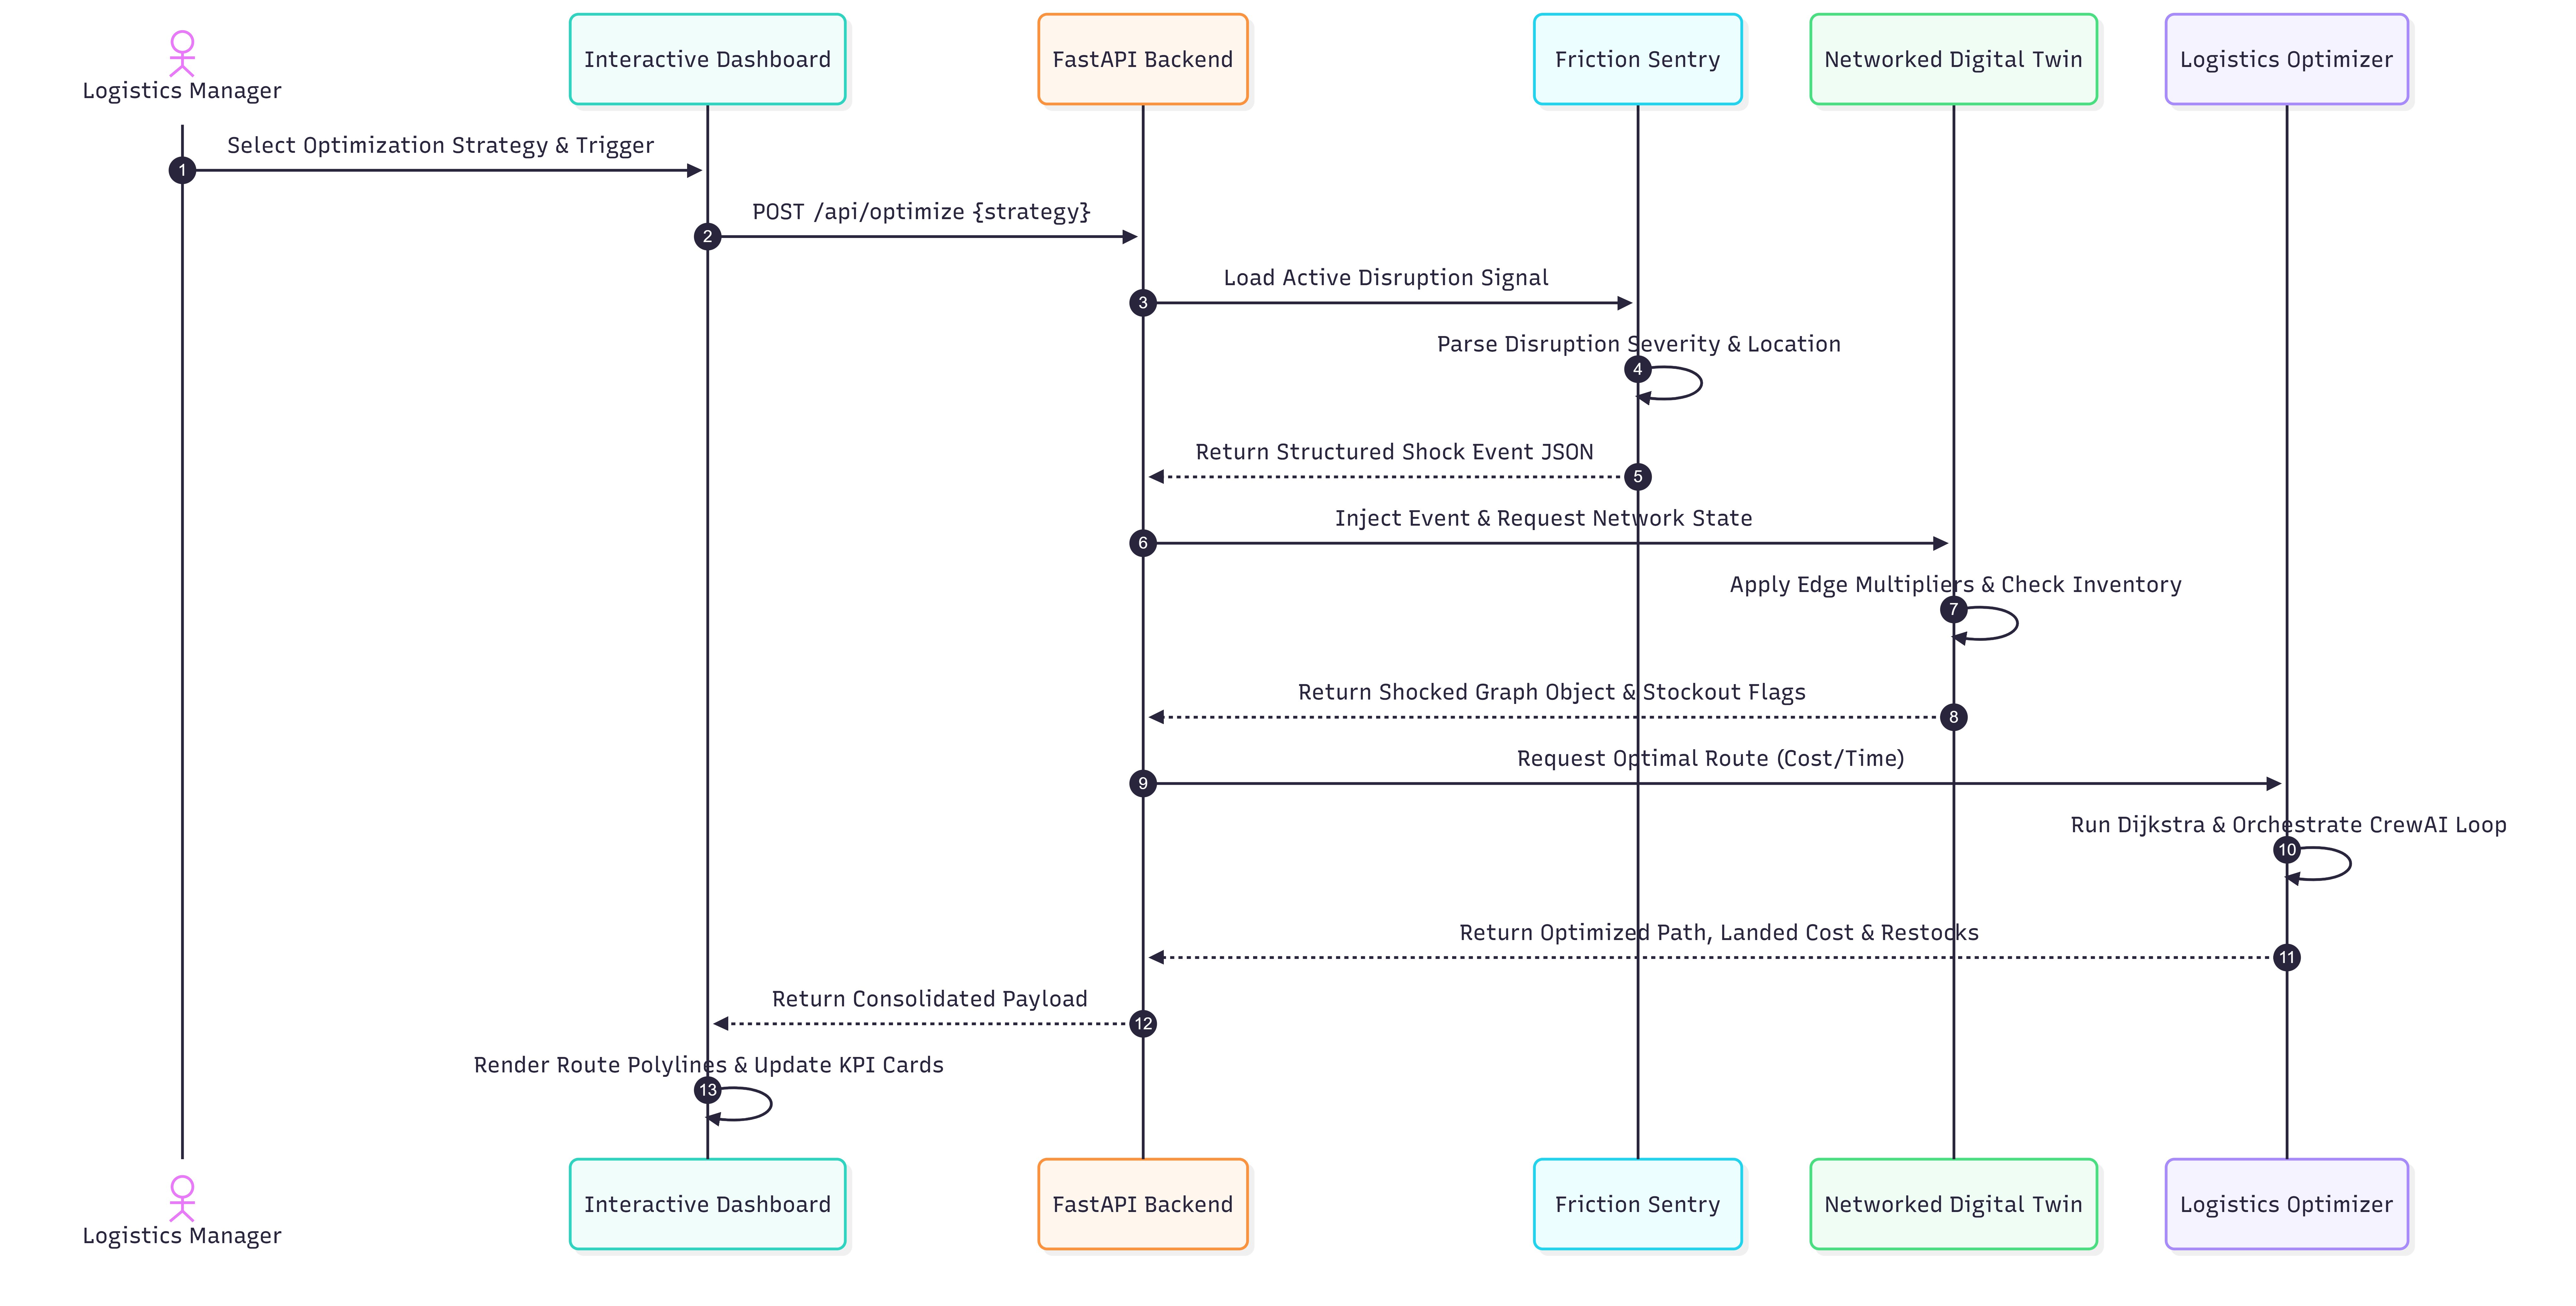
\includegraphics[width=\textwidth]{Figures/Interaction flow diagram.png}
    \caption{Detailed Module Interaction and Data Flow}
    \label{fig:interaction_flow}
\end{figure}

\begin{itemize}
    \item \textbf{Triggering of Operations:} System execution is event-triggered, initiated either by a simulated news alert or by the user selecting a strategic preference (cost/time) and clicking Run Optimization on the dashboard.
    \item \textbf{Data Exchange Flow:}
    \begin{enumerate}[label=(\roman*)]
        \item The API requests rules parsing.
        \item The parsed rules feed directly into the graph-modification engine to create a shocked state.
        \item The shocked state is evaluated for stockout risks.
        \item The shocked parameters and inventory metrics are passed as prompt context to the \texttt{CrewAI} reasoning agentic loop.
        \item The final dashboard payload is returned in a unified JSON structure.
    \end{enumerate}
\end{itemize}

\section[Module Description]{Module Description}
Detailed functional descriptions of each core module are provided in this section. For each module, the operational objective, inputs, internal processing steps, outputs, and dependencies are specified. This structured breakdown details the exact role that each module plays in the end-to-end simulation pipeline.

\subsection[Module 1: Friction Sentry]{Module 1: Friction Sentry}
\begin{itemize}
    \item \textbf{Module Name:} Friction Sentry
    \item \textbf{Objective/Purpose:} To ingest unstructured disruption logs and map them to standard risk variables and propagation parameters.
    \item \textbf{Inputs:}
    \begin{itemize}
        \item Raw event signal properties (location, event type, severity).
        \item Static translation database (\texttt{semantic\_mapping\_rules.json}).
    \end{itemize}
    \item \textbf{Internal Processing Performed:}
    \begin{itemize}
        \item Maps free-text locations to valid graph node IDs.
        \item Determines severity tiers (low, medium, high, critical) and extracts corresponding cost multipliers.
        \item Calculates cascaded disruptions to adjacent nodes using decay rates (e.g., cascading Strait of Hormuz shocks to Nhava Sheva port with a $0.50$ decay multiplier).
    \end{itemize}
    \item \textbf{Outputs:} Structured JSON shock event payload.
    \item \textbf{Dependencies:} \texttt{json}, \texttt{re}.
    \item \textbf{Interaction with Other Modules:} Feeds structured shock data directly into the Networked Digital Twin to apply edge changes.
\end{itemize}
The logical flow of signal processing and validation within the Friction Sentry is illustrated in Figure~\ref{fig:flow_friction_sentry}.

\subsubsection{Flowchart: Friction Sentry Module}
\begin{figure}[H]
\centering
\begin{tikzpicture}[scale=0.85, transform shape, node distance=1.1cm, every node/.style={align=center, font=\small},
    startstop/.style={rectangle, rounded corners=8pt, minimum width=3.5cm, minimum height=0.8cm, draw=black!80, fill=gray!10},
    process/.style={rectangle, minimum width=4.5cm, minimum height=0.8cm, draw=black!80, fill=white},
    decision/.style={diamond, aspect=2.5, minimum width=4cm, minimum height=0.8cm, draw=black!80, fill=gray!20},
    arrow/.style={->, thick}]
\node (start) [startstop] {Start: Receive Disruption Signal};
\node (loc) [process, below=of start] {Resolve Location to Node ID};
\node (type) [process, below=of loc] {Identify Signal Type and\\ Severity Tier};
\node (dec) [decision, below=of type] {Location\\Mapped?};
\node (calc) [process, below=of dec, yshift=-0.4cm] {Calculate Severity Multipliers\\and Cascade Decay Factors};
\node (out) [process, below=of calc] {Build Structured JSON\\Shock Payload};
\node (err) [process, right=3cm of dec] {Return Error:\\Unknown Node};
\node (dummy) [process, left=3cm of dec, draw=none, fill=none] {};
\node (end) [startstop, below=of out] {Output: Shock Payload\\to Digital Twin};
\draw[arrow] (start) -- (loc);
\draw[arrow] (loc) -- (type);
\draw[arrow] (type) -- (dec);
\draw[arrow] (dec) -- node[left]{Yes} (calc);
\draw[arrow] (dec) -- node[above]{No} (err);
\draw[arrow] (calc) -- (out);
\draw[arrow] (out) -- (end);
\end{tikzpicture}
\caption{Flowchart of Friction Sentry Module}
\label{fig:flow_friction_sentry}
\end{figure}

\subsection[Module 2: Networked Digital Twin]{Module 2: Networked Digital Twin}
\begin{itemize}
    \item \textbf{Module Name:} Networked Digital Twin
    \item \textbf{Objective/Purpose:} To simulate the impact of network shocks on transit lanes and track target market safety stock parameters.
    \item \textbf{Inputs:}
    \begin{itemize}
        \item Network topology configuration (\texttt{network\_topology.json}).
        \item Structured shock event payload (from Friction Sentry).
    \end{itemize}
    \item \textbf{Internal Processing Performed:}
    \begin{itemize}
        \item Modifies directed graph edge weights for cost and transit times according to severity multipliers.
        \item Evaluates inventory Days of Cover ($DoC$) for target markets.
        \item Executes the Chopra safety stock mathematical formulas to assess stock holding costs under lead time uncertainty.
        \item Checks if transit delay exceeds inventory cover to raise stockout flags.
    \end{itemize}
    \item \textbf{Outputs:} Shocked Network Graph Object (in-memory) and Inventory State Snapshot (utilization percentage, stockout Boolean).
    \item \textbf{Dependencies:} \texttt{networkx}, \texttt{InventoryManager} subclass.
    \item \textbf{Interaction with Other Modules:} Receives parameters from Friction Sentry and provides the active network state to the Logistics Optimizer for path-finding.
\end{itemize}
The step-by-step internal processing flow of the Networked Digital Twin, from shock ingestion through inventory assessment to graph output, is depicted in Figure~\ref{fig:flow_digital_twin}.

\subsubsection{Flowchart: Networked Digital Twin Module}
\begin{figure}[H]
\centering
\begin{tikzpicture}[scale=0.85, transform shape, node distance=1.1cm, every node/.style={align=center, font=\small},
    startstop/.style={rectangle, rounded corners=8pt, minimum width=3.5cm, minimum height=0.8cm, draw=black!80, fill=gray!10},
    process/.style={rectangle, minimum width=4.5cm, minimum height=0.8cm, draw=black!80, fill=white},
    decision/.style={diamond, aspect=2.5, minimum width=4cm, minimum height=0.8cm, draw=black!80, fill=gray!20},
    arrow/.style={->, thick}]
\node (start) [startstop] {Start: Receive Shock Payload};
\node (load) [process, below=of start] {Load Baseline Graph Topology};
\node (inject) [process, below=of load] {Inject Shock:\\Scale Edge Weights};
\node (inv) [process, below=of inject] {Calculate Inventory DoC\\and Safety Stock (Chopra)};
\node (dec) [decision, below=of inv, yshift=-0.4cm] {Delay $>$ DoC\\Buffer?};
\node (flag) [process, below right=0.6cm and 1.5cm of dec] {Set Stockout\\Flag = True};
\node (ok) [process, below left=0.6cm and 1.5cm of dec] {Inventory\\Status: Stable};
\node (out) [process, below=2.5cm of dec] {Output: Shocked Graph\\+ Inventory Snapshot};
\node (end) [startstop, below=of out] {Send to Logistics Optimizer};
\draw[arrow] (start) -- (load);
\draw[arrow] (load) -- (inject);
\draw[arrow] (inject) -- (inv);
\draw[arrow] (inv) -- (dec);
\draw[arrow] (dec.east) -| node[above,xshift=-0.5cm]{Yes} (flag.north);
\draw[arrow] (dec.west) -| node[above,xshift=0.5cm]{No} (ok.north);
\draw[arrow] (flag.south) |- (out.east);
\draw[arrow] (ok.south) |- (out.west);
\draw[arrow] (out) -- (end);
\end{tikzpicture}
\caption{Flowchart of Networked Digital Twin Module}
\label{fig:flow_digital_twin}
\end{figure}

\subsection[Module 3: Logistics Optimizer]{Module 3: Logistics Optimizer}
\begin{itemize}
    \item \textbf{Module Name:} Logistics Optimizer
    \item \textbf{Objective/Purpose:} To resolve network bottlenecks by computing optimal alternate paths and executing emergency inventory restocking actions.
    \item \textbf{Inputs:}
    \begin{itemize}
        \item Shocked Network Graph Object and Target Destination ID.
        \item Optimization Strategy selection (\texttt{cost} or \texttt{time}).
        \item Remote LLM Connection (via Gemini API).
    \end{itemize}
    \item \textbf{Internal Processing Performed:}
    \begin{itemize}
        \item Executes Dijkstra's algorithm to find alternate paths that bypass blocked chokepoints.
        \item Orchestrates a \texttt{CrewAI} execution pipeline (Logistics Solver $\rightarrow$ Cost Analyst $\rightarrow$ UX Communicator).
        \item Triggers the \texttt{EmergencyRestockTool} to inject replenishment inventory if analyst agents identify an imminent stockout.
        \item Benchmarks the dynamic optimized route against a static human baseline (subject to the Cost of Inaction).
    \end{itemize}
    \item \textbf{Outputs:} Optimized alternate route sequence, recalculated landed costs, optimized transit days, restock logs, and benchmark metrics.
    \item \textbf{Dependencies:} \texttt{crewai}, \texttt{networkx}, \texttt{google-genini-sdk}.
    \item \textbf{Interaction with Other Modules:} Receives graph structures from the Networked Digital Twin and sends calculation results to the Interactive Dashboard via API.
\end{itemize}
The end-to-end decision logic of the Logistics Optimizer, spanning Dijkstra routing, CrewAI agent orchestration, emergency restocking, and baseline benchmarking, is illustrated in Figure~\ref{fig:flow_optimizer}.

\subsubsection{Flowchart: Logistics Optimizer Module}
\begin{figure}[H]
\centering
\begin{tikzpicture}[scale=0.85, transform shape, node distance=1.1cm, every node/.style={align=center, font=\small},
    startstop/.style={rectangle, rounded corners=8pt, minimum width=3.5cm, minimum height=0.8cm, draw=black!80, fill=gray!10},
    process/.style={rectangle, minimum width=4.5cm, minimum height=0.8cm, draw=black!80, fill=white},
    decision/.style={diamond, aspect=2.5, minimum width=4cm, minimum height=0.8cm, draw=black!80, fill=gray!20},
    arrow/.style={->, thick}]
\node (start) [startstop] {Start: Receive Shocked Graph};
\node (dijk) [process, below=of start] {Run Dijkstra's Algorithm\\on Shocked Graph};
\node (dec1) [decision, below=of dijk, yshift=-0.4cm] {Path\\Found?};
\node (nopath) [process, right=2.5cm of dec1] {Activate Fallback:\\Return Direct Path};
\node (crew) [process, below=of dec1, yshift=-0.5cm] {Launch CrewAI Pipeline:\\Optimizer $\to$ Analyst $\to$ Communicator};
\node (dec2) [decision, below=of crew, yshift=-0.4cm] {Stockout\\Risk?};
\node (restock) [process, right=2.5cm of dec2] {Trigger Emergency\\Restocking Tool};
\node (bench) [process, below=of dec2, yshift=-0.5cm] {Benchmark AI vs.\\Human Baseline (CoI)};
\node (out) [process, below=of bench] {Compile Optimised\\Recommendation Payload};
\node (end) [startstop, below=of out] {Send to Dashboard via API};
\draw[arrow] (start) -- (dijk);
\draw[arrow] (dijk) -- (dec1);
\draw[arrow] (dec1.east) -- node[above]{No} (nopath);
\draw[arrow] (dec1) -- node[left]{Yes} (crew);
\draw[arrow] (nopath.south) |- (bench);
\draw[arrow] (crew) -- (dec2);
\draw[arrow] (dec2.east) -- node[above]{Yes} (restock);
\draw[arrow] (dec2) -- node[left]{No} (bench);
\draw[arrow] (restock.south) |- (bench);
\draw[arrow] (bench) -- (out);
\draw[arrow] (out) -- (end);
\end{tikzpicture}
\caption{Flowchart of Logistics Optimizer Module}
\label{fig:flow_optimizer}
\end{figure}

\subsection[Module 4: Interactive Dashboard]{Module 4: Interactive Dashboard}
\begin{itemize}
    \item \textbf{Module Name:} Interactive Dashboard
    \item \textbf{Objective/Purpose:} To provide a visual user interface mapping spatial route modifications, telemetry data, and comparative benchmark results.
    \item \textbf{Inputs:}
    \begin{itemize}
        \item Geographic coordinates dictionary (\texttt{COORDS}).
        \item Optimization payload containing routes, metrics, and stockout statuses.
    \end{itemize}
    \item \textbf{Internal Processing Performed:}
    \begin{itemize}
        \item Translates node ID chains into latitude/longitude sequences.
        \item Draws routing polylines (dashed for baseline routes, solid color-coded lines for optimized reroutes).
        \item Renders alert banners, metric widgets (landed cost comparison, transit time changes), and stockout logs.
    \end{itemize}
    \item \textbf{Outputs:} Interactive geographical web dashboard interface.
    \item \textbf{Dependencies:} \texttt{React}, \texttt{react-leaflet}, \texttt{axios}, \texttt{lucide-react}, \texttt{framer-motion}.
    \item \textbf{Interaction with Other Modules:} Triggers operations by sending optimization requests to the FastAPI backend and displays processing outcomes returned by the Logistics Optimizer.
\end{itemize}
The user interaction cycle of the Interactive Dashboard, from strategy selection and API dispatch through response validation to map and metric rendering, is shown in Figure~\ref{fig:flow_dashboard}.

\subsubsection{Flowchart: Interactive Dashboard Module}
\begin{figure}[H]
\centering
\begin{tikzpicture}[scale=0.85, transform shape, node distance=1.1cm, every node/.style={align=center, font=\small},
    startstop/.style={rectangle, rounded corners=8pt, minimum width=3.5cm, minimum height=0.8cm, draw=black!80, fill=gray!10},
    process/.style={rectangle, minimum width=4.5cm, minimum height=0.8cm, draw=black!80, fill=white},
    decision/.style={diamond, aspect=2.5, minimum width=4cm, minimum height=0.8cm, draw=black!80, fill=gray!20},
    arrow/.style={->, thick}]
\node (start) [startstop] {Start: Dashboard Load};
\node (map) [process, below=of start] {Render Geospatial Map\\with Baseline Routes};
\node (wait) [process, below=of map] {User Selects Strategy\\(Cost / Time)};
\node (click) [process, below=of wait] {User Clicks: Run Optimisation};
\node (post) [process, below=of click] {POST Request to\\/api/optimize};
\node (recv) [process, below=of post] {Receive JSON Payload\\from Backend};
\node (dec) [decision, below=of recv, yshift=-0.4cm] {Valid Response\\Received?};
\node (err) [process, right=2.5cm of dec] {Display Error\\Alert Banner};
\node (render) [process, below=of dec, yshift=-0.5cm] {Update Map Routes,\\Metric Cards, Summary};
\node (end) [startstop, below=of render] {Dashboard Updated:\\Await Next User Action};
\draw[arrow] (start) -- (map);
\draw[arrow] (map) -- (wait);
\draw[arrow] (wait) -- (click);
\draw[arrow] (click) -- (post);
\draw[arrow] (post) -- (recv);
\draw[arrow] (recv) -- (dec);
\draw[arrow] (dec.east) -- node[above]{No} (err);
\draw[arrow] (dec) -- node[left]{Yes} (render);
\draw[arrow] (err.south) |- (end.east);
\draw[arrow] (render) -- (end);
\end{tikzpicture}
\caption{Flowchart of Interactive Dashboard Module}
\label{fig:flow_dashboard}
\end{figure}

\section[Database and Interface Design]{Database and Interface Design}
The database and interface designs of the proposed system are detailed in this section. Managing a digital twin requires both structured document storage for network graphs and transactional flat-file recording for benchmark telemetry. The data organization strategies and user interface designs are described below.
\subsection[Database Design]{Database Design}
The system implements a hybrid data storage strategy tailored for digital twins and graph-theoretic applications.

\begin{itemize}
    \item \textbf{Database Type:} The project utilizes a NoSQL Document Store (JSON configuration files) for managing the network graph structure and configuration rules, combined with a Flat-File Relational Database (CSV format) for logging analytical, tabular benchmark statistics.
    \item \textbf{Data Organization Strategy:}
    \begin{itemize}
        \item \textbf{Network Topology Store (\texttt{network\_topology.json}):} Formatted as a document store modeling a directed graph, organizing data into nodes (entities) and edges (relational links).
        \item \textbf{Semantic Rules Library (\texttt{semantic\_mapping\_rules.json}):} Stores risk factors and propagation properties as structured, hierarchical key-value documents.
        \item \textbf{Comparative Analysis Log (\texttt{comparative\_analysis.csv}):} Stores structured, flat-file relational records comparing execution metrics of human vs. AI agents for dashboard ingestion.
    \end{itemize}
    \item \textbf{Relationships between Entities:}
    \begin{itemize}
        \item \textbf{Nodes and Edges:} A node represents a physical facility (Supplier, Port, Warehouse, or Market). Edges represent directional shipping lanes connecting a source node to a target node, containing attributes like baseline cost, baseline transit time, and mode.
        \item \textbf{Events and Nodes:} A disruption event maps directly to one or more nodes (representing the location of the shock) and propagates along outgoing edges.
    \end{itemize}
    \item \textbf{Storage Structure:} In-memory representation uses Python dictionary mappings and dynamic NetworkX graph structures, backed by persistent local file storage to minimize database connection overheads and maximize execution speed.
\end{itemize}

\subsection[ER Diagram]{ER Diagram}
The following diagram illustrates the logical relationships between the core operational entities modeled in the logistics digital twin:

\begin{figure}[htbp]
    \centering
    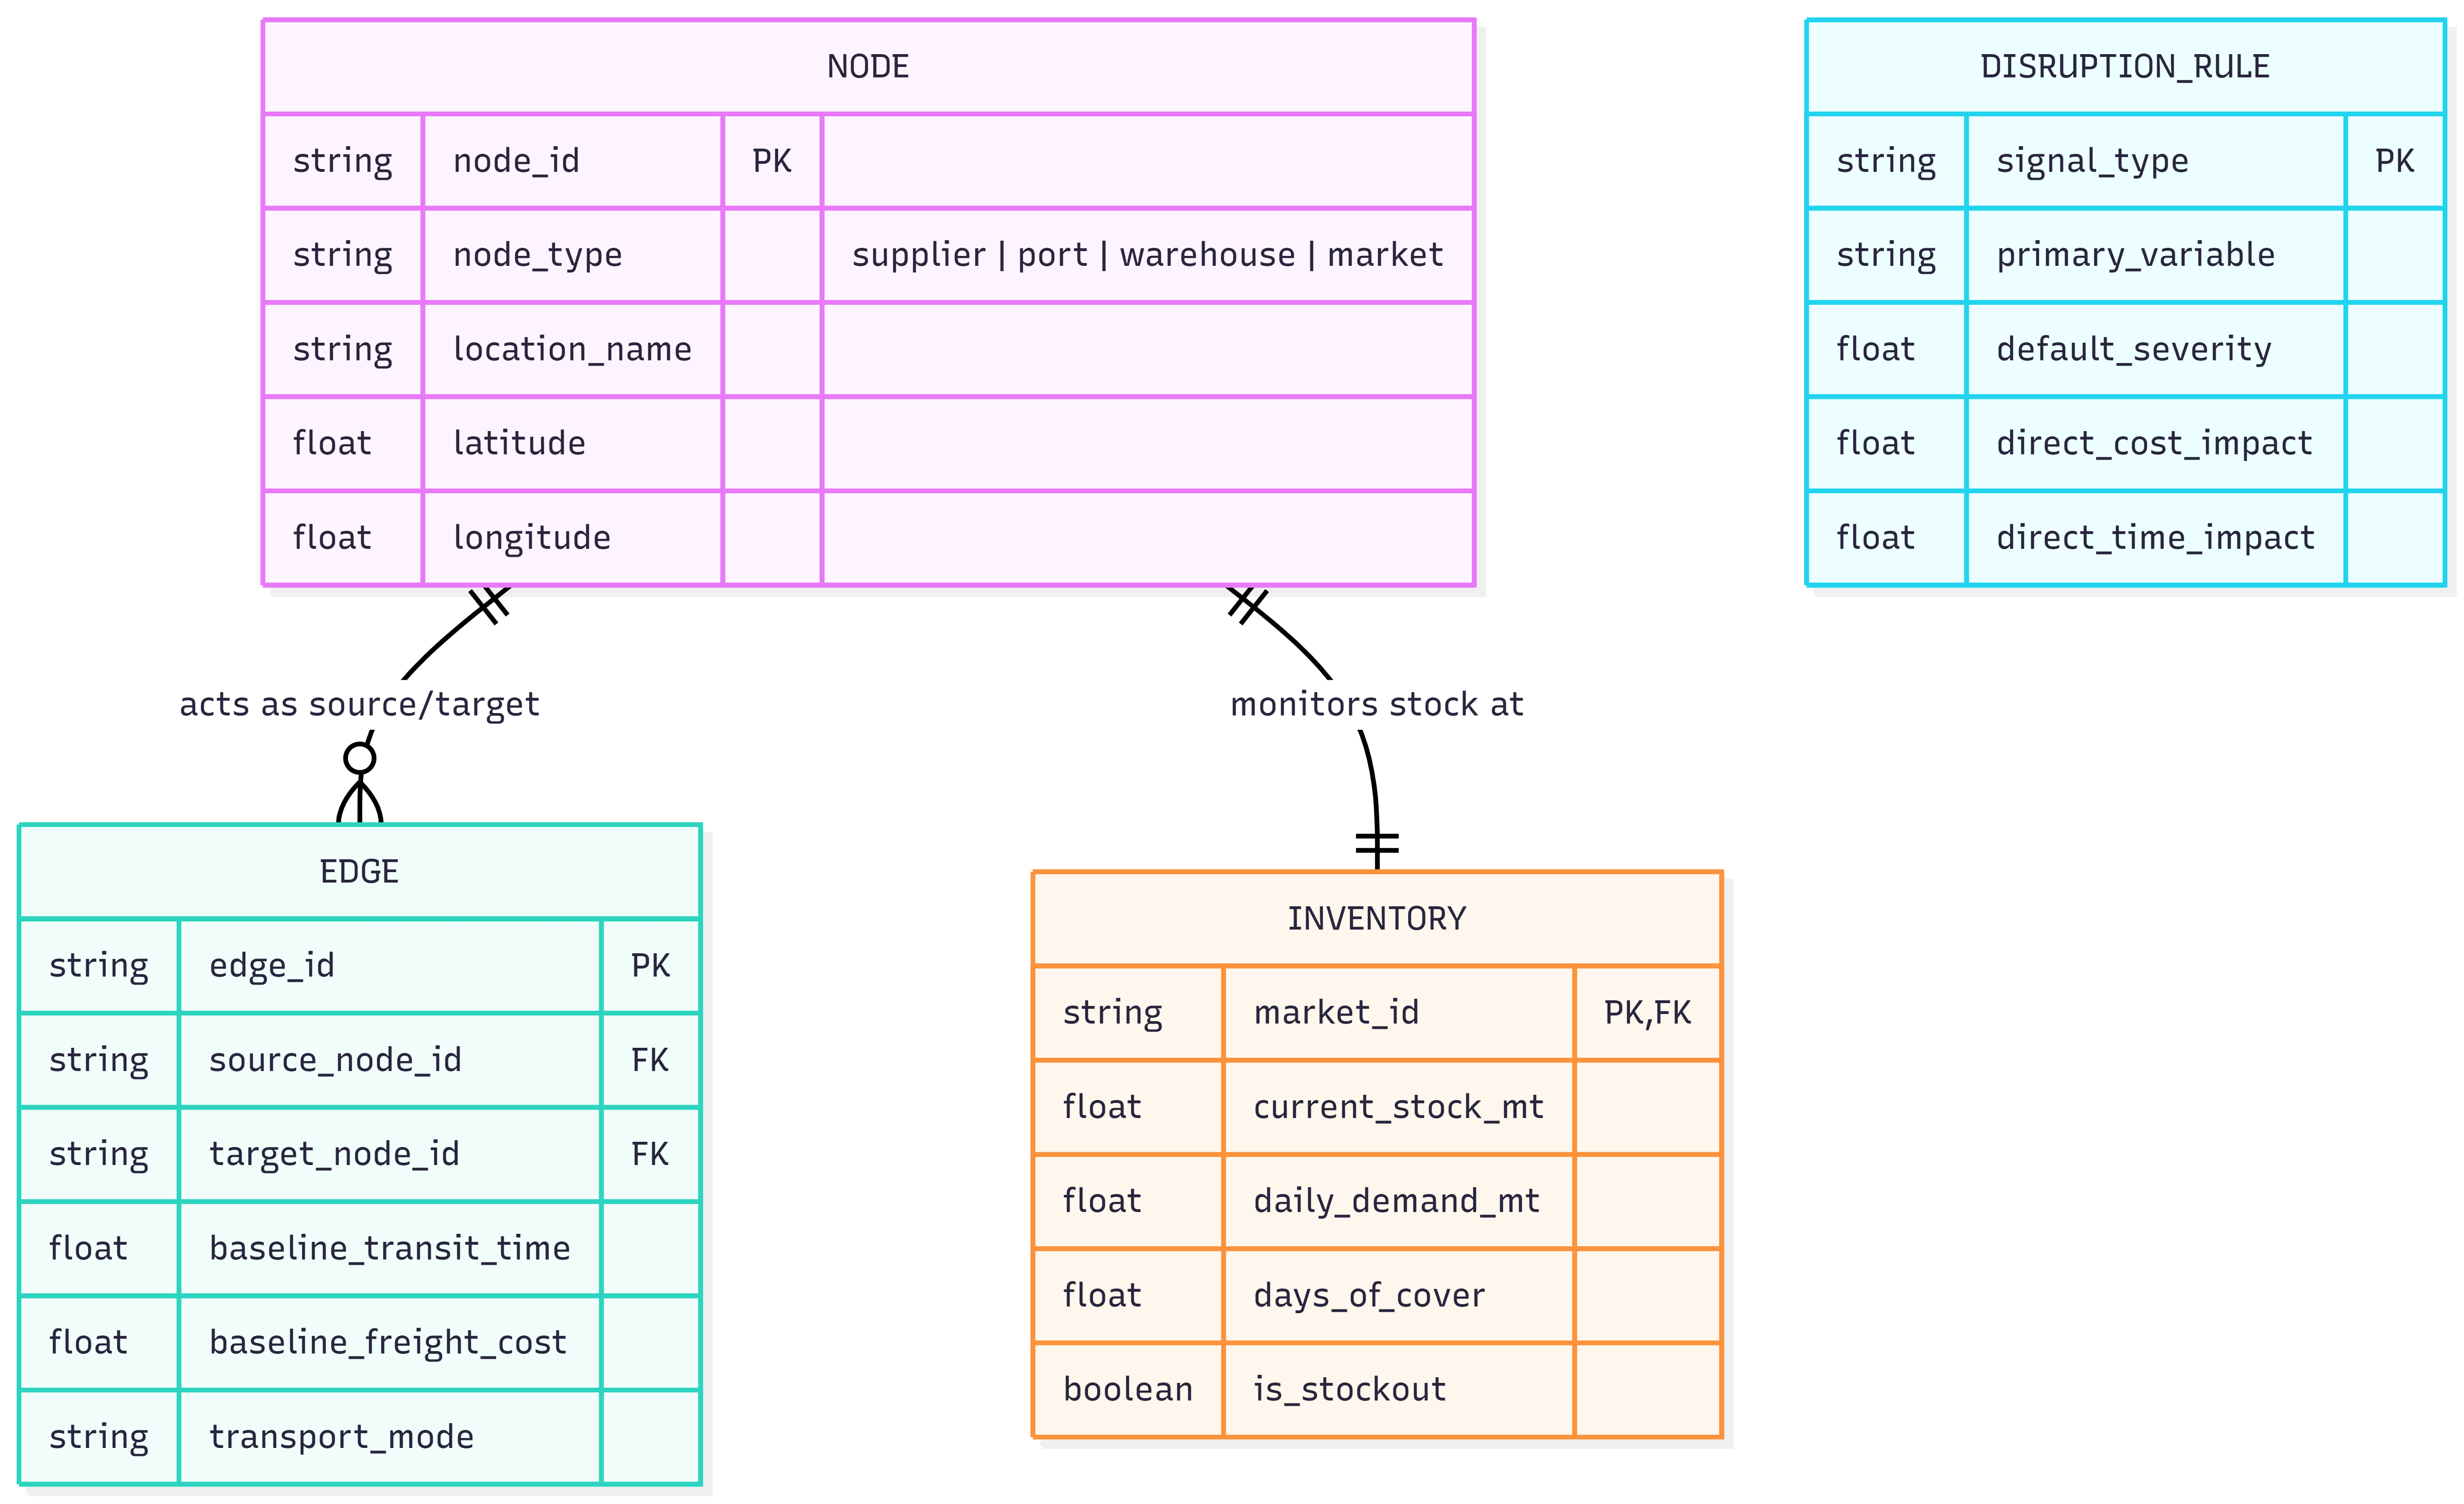
\includegraphics[width=\textwidth]{Figures/ERD.png}
    \caption{Entity-Relationship Diagram for Logistics Digital Twin}
    \label{fig:erd}
\end{figure}

\subsection[Table Structure Description]{Table Structure Description}

\subsubsection{Entity: NODE}
\textbf{Purpose:} Defines physical facilities and processing nodes within the logistics network, as shown in Table \ref{tab:node_structure}
\begin{table}[htbp]
\centering
\caption{Node Entity Structure}
\label{tab:node_structure}
\resizebox{\textwidth}{!}{
\begin{tabular}{|l|l|l|l|}
\hline
\textbf{Field Name} & \textbf{Data Type} & \textbf{Constraints} & \textbf{Field Purpose} \\ \hline
\texttt{id} & String & Primary Key, Unique, Not Null & Unique identifier for the network node (e.g., \texttt{nhava\_sheva}). \\ \hline
\texttt{type} & String & Enums: \texttt{supplier}, \texttt{port}, \texttt{warehouse}, \texttt{market} & Categorizes the operational nature of the facility. \\ \hline
\texttt{name} & String & Not Null & User-friendly geographical name (e.g., Nhava Sheva Port). \\ \hline
\texttt{latitude} & Float & Range: $-90.0$ to $90.0$ & Latitude coordinate for geographical mapping. \\ \hline
\texttt{longitude} & Float & Range: $-180.0$ to $180.0$ & Longitude coordinate for geographical mapping. \\ \hline
\end{tabular}
}
\end{table}

\subsubsection{Entity: EDGE}
\textbf{Purpose:} Represents shipping lanes connecting physical nodes in the graph, as shown in Table \ref{tab:edge_structure}.

\begin{table}[htbp]
\centering
\caption{Edge Entity Structure}
\label{tab:edge_structure}
\resizebox{\textwidth}{!}{
\begin{tabular}{|l|l|l|l|}
\hline
\textbf{Field Name} & \textbf{Data Type} & \textbf{Constraints} & \textbf{Field Purpose} \\ \hline
\texttt{source} & String & Foreign Key (references \texttt{NODE.id}) & Origin node of the logistics lane. \\ \hline
\texttt{target} & String & Foreign Key (references \texttt{NODE.id}) & Destination node of the logistics lane. \\ \hline
\texttt{transit\_time} & Float & Value $>$ 0 & Baseline duration in days to traverse the lane. \\ \hline
\texttt{freight\_cost} & Float & Value $>$ 0 & Baseline transportation cost in USD. \\ \hline
\texttt{mode} & String & Enums: \texttt{ocean}, \texttt{road}, \texttt{rail} & Transport modality utilized on the lane. \\ \hline
\end{tabular}
}
\end{table}

\subsubsection{Entity: INVENTORY}
\textbf{Purpose:} Tracks real-time stock parameters for destination nodes, as shown in Table \ref{tab:inventory_structure}.

\begin{table}[htbp]
\centering
\caption{Inventory Entity Structure}
\label{tab:inventory_structure}
\resizebox{\textwidth}{!}{
\begin{tabular}{|l|l|l|l|}
\hline
\textbf{Field Name} & \textbf{Data Type} & \textbf{Constraints} & \textbf{Field Purpose} \\ \hline
\texttt{market\_id} & String & Primary Key, Foreign Key (references \texttt{NODE.id}) & Identifies which market the inventory parameters apply to. \\ \hline
\texttt{current\_stock\_mt} & Float & Value $\geq$ 0 & Quantity of stock currently on hand in Metric Tons. \\ \hline
\texttt{daily\_demand\_mt} & Float & Value $>$ 0 & Average daily inventory consumption rate. \\ \hline
\texttt{days\_of\_cover} & Float & Value $\geq$ 0 & Estimated days remaining before stock is fully depleted. \\ \hline
\texttt{is\_stockout} & Boolean & True / False & Flag showing whether on-hand inventory is completely depleted. \\ \hline
\end{tabular}
}
\end{table}

\subsection[Interface Design]{Interface Design}

The user interface is designed as an interactive, single-page command-and-control dashboard structured to visualize real-time simulation data.

\begin{itemize}
    \item \textbf{Screen Organization:} \\
    The layout is divided into three primary visual zones:
    \begin{enumerate}[label=\alph*)]
        \item \textbf{Top Banner (Notification Panel):} Renders critical shock alerts (e.g., location, event type, severity multiplier) detected by the Friction Sentry.
        \item \textbf{Left Panel (Geospatial Digital Twin Map):} Displays two visual maps in a split container: the \textit{Baseline Network Map} showing undisrupted transit routes, and the \textit{Optimized Alternate Route Map} highlighting the new routing paths calculated by the system.
        \item \textbf{Right Panel (Control and Telemetry Panel):} Hosts the strategy configuration controls, optimization triggers, and dynamic performance cards (e.g., Transit Time Delta, Cost Delta, Stockout Alarms, Executive Summaries).
    \end{enumerate}
    \item \textbf{Navigation Flow:} \\
    As a Single Page Application (SPA), the user does not leave the dashboard. The navigation flow is structural:
    \begin{center}
        \small
        Dashboard Load $\rightarrow$ Dynamic Map Renders $\rightarrow$ Configure Strategy (Cost/Time) $\rightarrow$ \\
        Click 'Run Optimization' $\rightarrow$ Executive Summary Slides In $\rightarrow$ Path Update Animates on Map
    \end{center}
    \item \textbf{Input Forms / Control Elements:}
    \begin{itemize}
        \item \textbf{Strategy Toggle:} Radio buttons allow the user to select the optimization objective (\texttt{Minimize Cost} vs. \texttt{Minimize Time}).
        \item \textbf{Action Button:} A single high-contrast button labeled \texttt{Run Optimization} triggers the background agentic pipeline.
    \end{itemize}
    \item \textbf{Output Displays:}
    \begin{itemize}
        \item \textbf{Alert Banner:} Dynamic color-coded notifications showing active network shocks (e.g., Verification Delay: Multiplier 1.35x).
        \item \textbf{Dynamic Map Overlay:} Renders physical nodes (markers) and interactive polylines (dashed gray for baseline routes, bold purple for optimized agent routes).
        \item \textbf{Metric Cards:} Renders computed values for the optimized paths, including \textit{New Transit Days} and \textit{Cost Delta}.
        \item \textbf{Executive Summary:} A dynamic text block generated by the Communicator Agent explaining the reasoning behind the recommended actions.
    \end{itemize}
\end{itemize}

\subsection[API / Module Interface Design]{API / Module Interface Design}

The system facilitates module communication via a RESTful API layer managed by FastAPI using standardized JSON payloads.

\subsubsection{API Interaction Workflow}
\begin{itemize}
    \item Communication between the React client and FastAPI server is handled over HTTP/HTTPS using standard CRUD operations.
    \item Dynamic optimization queries use \texttt{POST} requests containing configuration parameters in the request body.
\end{itemize}

\subsubsection{Request-Response Structure}

\textbf{A. Shock Detection Endpoint (\texttt{GET /api/shock})}
\begin{itemize}
    \item \textbf{Purpose:} Retrieves the active network shock parsed by the Friction Sentry.
    \item \textbf{Response Format (JSON):}
\end{itemize}

\textbf{B. Optimization Trigger Endpoint (\texttt{POST /api/optimize})}
\begin{itemize}
    \item \textbf{Purpose:} Runs the multi-agent optimization sequence based on user preference.
    \item \textbf{Request Body (JSON):}
\end{itemize}
\begin{lstlisting}[language=json,numbers=none]
{
  "optimize_by": "cost"
}
\end{lstlisting}
\begin{itemize}
    \item \textbf{Response Format (JSON):}
\end{itemize}
\begin{lstlisting}[language=json,numbers=none]
{
  "recommended_path": "oman -> nhava_sheva -> mumbai_warehouse -> bengaluru_sme_market",
  "total_transit_days": 10.34,
  "total_cost_usd": 1695.96,
  "reroute_triggered": true,
  "summary_text": "AI selected the Oman-to-Bengaluru path via Nhava Sheva to avoid Red Sea shocks. Landed cost optimized to $1,695.96 with a 10.34-day transit delay.",
  "delta": {
    "time_change": "10.34 days",
    "cost_increase": "+$0.00"
  }
}
\end{lstlisting}

\subsubsection{Communication Interfaces}
\begin{itemize}
    \item \textbf{CORS Middleware:} Backend APIs are configured with Cross-Origin Resource Sharing (CORS) policies to allow communication from the local React frontend port (e.g., \texttt{http://localhost:5173}).
    \item \textbf{Data Exchange Format:} All data exchanges are formatted as strict \textbf{application/json} payloads. Client-side state updates are triggered asynchronously upon resolution of the HTTP request promise.
\end{itemize}

\section[Detailed Workflow and Processing]{Detailed Workflow and Processing}
This section presents the detailed workflow and processing routines executed by the system during a simulation run. The lifecycle of a request involves input acquisition, validation, graph transformation, agentic reasoning, and output serialization. These sequential stages are explained in detail in the following subsections.

\subsection[Input Processing Workflow]{Input Processing Workflow}
This subsection details how incoming requests and disruption signals are parsed and validated:

\begin{itemize}
    \item \textbf{Input Acquisition:} \\
    The system acquires inputs from two channels:
    \begin{enumerate}
        \item \textbf{User Action:} The frontend client transmits optimization preferences (e.g., \texttt{\{optimize\_by: cost\}}) via asynchronous HTTP POST requests.
        \item \textbf{External File Stream:} The Friction Sentry ingests shock events (event date, target node location, signal type, severity classification) from configuration inputs.
    \end{enumerate}
    \item \textbf{Input Validation:} \\
    Backend validation is handled programmatically at the API layer:
    \begin{itemize}
        \item \textbf{Type Enforcement:} Inputs are validated using Pydantic models (e.g., checking that \texttt{optimize\_by} matches one of the string constants \texttt{cost} or \texttt{time}).
        \item \textbf{Bounds Verification:} Severity multipliers are checked to ensure they are numeric values $\geq 1.0$.
    \end{itemize}
    \item \textbf{Input Formatting:} \\
    Incoming raw strings are stripped of whitespace and converted to standardized, lowercase system identifiers. For example, user inputs or news locations (e.g., Nhava Sheva) are mapped to graph node IDs (e.g., \texttt{nhava\_sheva}).
    \item \textbf{Data Verification:} \\
    Before executing calculations, the backend verifies that the requested shock location and target market IDs exist in the active \texttt{network\_topology.json} model to prevent reference key errors.
\end{itemize}

\subsection[Internal Processing Workflow]{Internal Processing Workflow}
This subsection details the processing stages executed once inputs are verified, as shown by Figure \ref{fig:impl}
\begin{figure}[htbp]
    \centering
    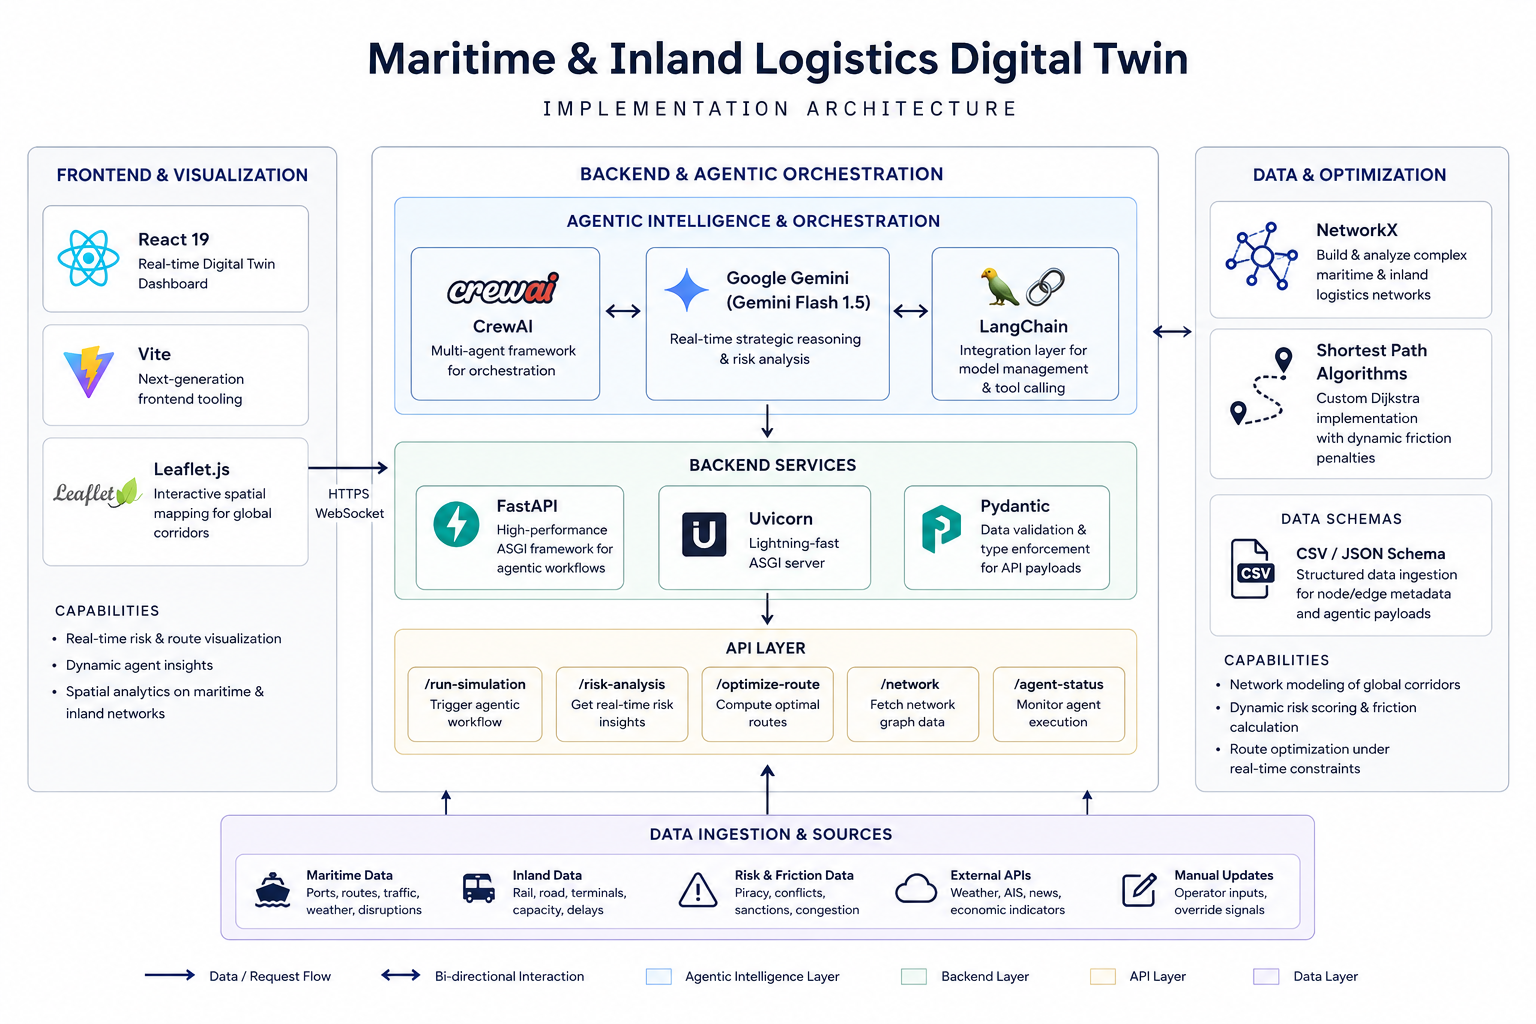
\includegraphics[width=0.9\textwidth]{Figures/impl.png}
    \caption{Internal Processing Workflow}
    \label{fig:impl}
\end{figure}
\begin{itemize}
    \item \textbf{Core Processing Stages:} \\
    The system executes a sequence of logical operations starting from input validation, injecting shock multipliers into the graph model, computing optimized paths via Dijkstra's algorithm, orchestrating the CrewAI reasoning loop, and performing final inventory health checks.

    
    \item \textbf{Internal Data Movement:}
    \begin{itemize}
        \item \textbf{Graph Model Loading:} The engine reads the baseline graph model and instantiates a \texttt{networkx.DiGraph} object.
        \item \textbf{Shock Injection:} Edge weights ($w_t$ and $w_c$) on the graph are scaled at the target locations using the shock severity multiplier.
        \item \textbf{Path Optimization:} Dijkstra's algorithm computes the shortest path arrays (sequence of node IDs) based on the current active weight.
        \item \textbf{Agent Prompt Construction:} The computed path sequences, delta days, and inventory snapshots are injected into the LLM system prompt templates for the CrewAI task configurations.
    \end{itemize}
    \item \textbf{Module Coordination and Sequence:} \\
    Execution follows a strict sequential pipeline:
    \begin{equation}
    \text{Friction Ingestion} \rightarrow \text{Graph Shock Calculation} \rightarrow \text{Dijkstra Routing} \rightarrow \text{Agentic Analysis and Stock Check} \rightarrow \text{Payload Consolidation}
    \end{equation}
\end{itemize}

\subsection[Output Generation Workflow]{Output Generation Workflow}
This subsection details how the backend formats and delivers results:

\begin{itemize}
    \item \textbf{Output Generation Process:} \\
    Upon completion of the agent tasks, the system coordinates the outputs of the \textit{Optimizer}, \textit{Analyst}, and \textit{Communicator} agents.
    \item \textbf{Data Formatting:} \\
    Raw agent logs are parsed using regular expressions to isolate the outermost JSON block. Float values (such as costs and days) are rounded to two decimal places. Path sequences are formatted as clean string links (e.g., \texttt{Node A -> Node B -> Node C}).
    \item \textbf{Notification or Response Generation:} \\
    FastAPI converts the internal dictionary objects into a JSON HTTP response payload. Concurrently, the system updates the terminal logging console. The frontend intercepts this payload to trigger animations and update map polylines.
\end{itemize}

\subsection[Exception and Validation Flow]{Exception and Validation Flow}
This subsection explains how the system handles operational errors and exception states:

\begin{itemize}
    \item \textbf{Validation Mechanisms:}
    \begin{itemize}
        \item \textbf{Pydantic Schemas:} Detects invalid parameters at the REST endpoint level, returning HTTP 422 Unprocessable Entity errors.
        \item \textbf{Reference Checks:} Custom validators verify that nodes parsed by the Friction Sentry exist in the active topology graph.
    \end{itemize}
    \item \textbf{Error Handling Flow:}
    \begin{itemize}
        \item \textbf{LLM API Timeout:} If the Google Gemini connection experiences high network latency or API rate limits, the system raises a connection timeout exception.
        \item \textbf{Graph Disconnection:} If a shock completely isolates a destination node (blocking all paths), Dijkstra's algorithm will fail to find a path, raising a \texttt{NetworkXNoPath} error.
    \end{itemize}
    \item \textbf{Recovery Mechanisms:}
    \begin{itemize}
        \item \textbf{Agent Route Fallback:} If the \texttt{CrewAI} process fails to output valid route JSON due to parser exceptions, the system activates a fallback handler that returns the mathematically computed Dijkstra path coordinates directly to the frontend.
        \item \textbf{Graceful API Degradation:} Under API errors, the UI replaces detailed summar" status ": " active ",
ies with predefined, simplified alert messages while maintaining graph rendering.
    \end{itemize}
\end{itemize}








\section[Summary]{Summary}
This chapter provided a Detailed Design of the logistics digital twin, focusing on internal module logic, database schemas, and interface structures. It translated high-level architectural goals into specific execution workflows and API contracts for the multi-agent system. These detailed specifications ensure a cohesive integration between the backend optimization engine and the interactive frontend dashboard.
